% =============================================================
% DataMind -- SIGMOD research-paper draft
% =============================================================

\section{Introduction}
\label{sec:intro}

A tool-using language model rarely answers a serious enterprise question from
its parameters alone. ReAct and Toolformer established the now-common pattern
of interleaving model reasoning with calls to external tools~\cite{yao2023react,schick2023toolformer};
multi-agent runtimes such as AutoGen make those calls composable across an
application~\cite{wu2024autogen}. In an enterprise workspace, the tools read a
policy document, inspect a table, follow a file dependency, or recall a
decision made earlier in a project. These artifacts form a workspace: a
collection of heterogeneous data products that is private to a user or team
and changes as work proceeds. The model is only one participant in this
setting. A data system must decide how the workspace is represented, which
representations are visible to a request, how an update is published, and how
an answer can be traced back to its sources.

This setting is different from a conventional retrieval-augmented generation
(RAG) application~\cite{lewis2020rag}. A document retriever can return
passages, and graph-oriented RAG can organize evidence around entities or
communities~\cite{edge2024graphrag}, but neither representation says whether a
database view was built from the same source revision. A text-to-SQL agent can
execute a query, while systems such as DB-GPT and SiriusBI focus on natural
language interaction with particular database or business-intelligence
workloads~\cite{xue2024dbgpt,jiang2025siriusbi}. They do not provide a policy
for combining a table result with a document assertion or a dependency edge.
A graph retriever can expose relationships, but it does not determine whether
the graph is stale while the corresponding files are being edited. Existing
agent runtimes and tool protocols make it easy to expose these components as
endpoints~\cite{wu2024autogen,mcp2025tools}; the semantics of the data exchanged
between them remain application-specific.

The problem becomes visible when the agent must first decide where to look.
Enterprise data-integration work has documented the gap between an LLM and the
private, heterogeneous data products used by organizations~\cite{kayali2025mindgap},
while pipeline-oriented systems such as AOP study how to compose operators
over structured and unstructured sources~\cite{wang2025aop}. WorkSurface-Bench
isolates the corresponding serving problem: it evaluates enterprise tasks over
document, table, graph, and cross-surface data, and reports routing, evidence,
answer, and efficiency separately~\cite{worksurfacebench2026}. Its controlled
settings show why surface selection is only one part of the problem: even when
the required surface is known, the agent still has to perform the right
operation and produce an answer supported by the returned evidence. A system
that exposes all sources as unrelated tools cannot express which sources form
one project, which revision should be read, or what evidence is safe to
combine.

We study the following data-management problem:

\begin{quote}
Given a mutable workspace and a set of agent requests, how can a system
materialize heterogeneous data surfaces, publish a consistent profile view,
and serve that view to agents with bounded routing, provenance, update, and
recovery semantics?
\end{quote}

We present \textbf{DataMind}, a profile-scoped multi-surface data plane for
tool-using agents. DataMind separates two roles that are often mixed together
in application code. A \emph{Build Agent} organizes raw workspace artifacts
into data surfaces: parsed and indexed documents, relational projections, and
dependency graphs. Profile and session memory is populated by the StoreAgent
through the same surface contracts. A \emph{Serving Agent} consumes a
published profile view, selects the surfaces and operations relevant to a
request, and returns values together with evidence receipts. Both roles use the
same profile, surface contract, revision, provenance, and policy metadata.

The central abstraction is a profile snapshot. A profile is the isolation
boundary for a user, project, or tenant. Its snapshot names the revisions of
the surfaces that a request is allowed to observe. A surface manifest describes
its schema, operations, source set, freshness, evidence type, access policy,
and estimated cost. Build operations produce source-linked receipts; serving
operations propagate those receipts into the answer trace. A build records a
candidate descriptor and advances the logical publication pointer only after
validation. The prototype blocks reads of surfaces touched by an active
candidate and fails closed when a live-only provider can no longer satisfy a
pinned request. This gives the system an explicit update boundary without
requiring every physical backend to implement the same storage model.
The design follows the provenance distinction between a result and its
derivation~\cite{cheney2009provenance,green2007provenance}, but applies it to
retrieval, SQL, graph traversal, and memory operations in one serving trace.

DataMind is not a new vector index, text-to-SQL model, graph algorithm, or
language model. Its contribution is a data-plane boundary around the external
state used during inference. The boundary allows an organization to retain its
existing parser, database, vector store, graph store, or ETL job while exposing
the resulting data products through a common profile and capability interface.
It also gives local IDE agents and hosted runtimes the same data semantics;
MCP, native loops, and SDKs are adapters at the edge of the plane.

We evaluate the two directions of the plane separately and together.
WorkSurface-Bench is the main serving workload: it measures routing, evidence,
answer quality, and efficiency under a fixed tool protocol~\cite{worksurfacebench2026}.
WorkSurface-Build
starts from raw workspace artifacts and measures materialization cost and the
downstream value of the resulting surfaces. Additional workloads exercise
incremental changes, concurrent requests, profile isolation, and failures of
parsers, indexes, databases, and graphs. The goal is to measure not only
whether an agent answers a question, but whether the answer remains reproducible
as the workspace evolves.

This paper makes three contributions:
\begin{itemize}
  \item We formulate workspace interaction as a profile-scoped
  multi-surface data-management problem with explicit contracts for surface
  operations, revision visibility, provenance, evidence, and policy.
  \item We design and implement DataMind, a build--serve runtime that
  materializes, publishes, routes, and updates document, relational, graph,
  and memory surfaces for tool-using agents, with explicit stale-read and
  candidate-build failure semantics.
  \item We combine an auditable multi-surface serving workload with build,
  update, concurrency, and failure experiments, separating agent quality from
  the data-system costs and correctness properties that support it.
\end{itemize}

\section{Problem Setting}
\label{sec:problem}

\subsection{Workspaces and data surfaces}
\label{sec:workspace}

A workspace $W$ contains source artifacts $a_1,\ldots,a_n$. An artifact can be
a document, spreadsheet, database record, source file, generated report, or
user-provided memory item. A \emph{surface} is a materialized representation
of a subset of $W$ together with a family of operations that an agent can
invoke. We consider four surfaces:
\begin{itemize}
  \item a \textbf{document surface} with parsed blocks, chunks, embeddings,
  lexical indexes, and source locators;
  \item a \textbf{database surface} with typed tables or views and executable
  relational operations;
  \item a \textbf{graph surface} with entities, edges, and source annotations
  for dependency and relationship queries; and
  \item a \textbf{memory surface} with scoped records that persist project or
  user state across sessions.
\end{itemize}

The surfaces are complementary rather than mutually exclusive. A project
report can yield passages for a document index, rows for a relational view,
and an edge connecting the report to a code artifact. Treating each result as
an independent tool loses this common origin. DataMind therefore associates
source identifiers and checksums with derived records and exposes the relation
between a result and the surface that produced it.

\subsection{Profiles and snapshots}
\label{sec:profile-snapshot}

A profile $p$ binds a workspace, source roots, access policy, surface
manifests, and persistent state. Profiles provide the boundary required for
local projects and multi-tenant services: a request in profile $p$ must not
implicitly read a source or memory item belonging to $p'$. A profile may also
contain session state, but session state is a narrower scope than profile state
and does not change the profile's durable data products.

For each surface $s$, a build produces a revision $r_s$. A snapshot $\sigma_p$
is a persistent publication record containing a vector of visible revisions:
\[
  \sigma_p = \langle r_{\mathrm{doc}}, r_{\mathrm{db}},
  r_{\mathrm{graph}}, r_{\mathrm{memory}} \rangle .
\]
A serving request is evaluated against $(p,\sigma_p)$. The publication record
is advanced only after candidate validation. The built-in prototype providers
currently expose a live view rather than historical artifact files. Reads for
surfaces touched by an active candidate are blocked, and if a request's pinned
record is superseded while it is running, the runtime fails closed instead of
silently combining revisions. This explicit boundary keeps
the logical snapshot contract useful while making the provider limitation
observable and measurable.

\subsection{Surface contracts}
\label{sec:surface-contract}

Each surface exposes a manifest
\[
 M_s=(\mathit{schema},\mathit{ops},\mathit{sources},\mathit{revision},
 \mathit{freshness},\mathit{evidence},\mathit{policy},\mathit{cost}).
\]
The schema describes the shape of values and locators. Operations describe
what the Serving Agent can do, such as lexical or vector retrieval, SQL
execution, or graph traversal. Freshness and revision describe when the result
was produced. Evidence describes how a result can be cited: a document span, a
query and returned rows, or a graph path with source edges. Cost summarizes
latency, token transfer, and optional external-service cost. Policy states the
profile and operation constraints.

The manifest is used in both directions. The Build Agent uses it to declare
what a materialization will contain and which source artifacts it covers. The
Serving Agent uses it to eliminate operations whose schema, scope, or evidence
type cannot satisfy a request. This is a data-system interface: it keeps the
model-facing operation stable while allowing a surface to change its physical
index or storage implementation.

\subsection{Receipts and evidence}
\label{sec:receipts}

A write receipt records the profile, source reference, surface operation,
revision, item count, and status. A read evidence receipt records the profile,
snapshot, surface, source identifier, locator, and returned value. A response
may contain several receipts when a question requires a document, a database,
and a graph operation. The receipt set is the system's explanation of which
materialized facts were available to the generator; it is not a post-hoc
similarity score.

This design follows the database provenance distinction between a result and
its derivation~\cite{cheney2009provenance,green2007provenance}, while adapting
the unit of provenance to heterogeneous Agent operations. The prototype does
not claim tuple-level provenance for every physical backend. It does claim
that each DataMind operation identifies the source and revision it exposes,
and that the request trace preserves the operations used to form the answer.

\subsection{Build, serve, and maintenance goals}
\label{sec:goals}

The system is designed around five goals:
\begin{enumerate}
  \item \textbf{Materialization}: organize heterogeneous artifacts into
  complementary surfaces while retaining source identity;
  \item \textbf{Serving}: choose and compose surface operations without
  requiring the model to copy large intermediate results through its context;
  \item \textbf{Visibility}: make updates observable at a defined revision and
  keep a request on its selected snapshot;
  \item \textbf{Isolation}: carry profile and policy through every read and
  write; and
  \item \textbf{Recovery}: distinguish an empty result from an unavailable
  surface and resume or fall back without silently losing evidence.
\end{enumerate}

\section{DataMind Data Plane}
\label{sec:system}

DataMind is the complete data plane between a mutable workspace and a
tool-using Agent. It has two logically separate paths that share the same
profile, surface contracts, provenance, policy, and revision semantics.
Figure~\ref{fig:datamind-overview} is the serving view: it shows how a request
is routed over already materialized surfaces and returned with evidence. The
corresponding ingestion path is DataMind-Build, shown in
Figure~\ref{fig:datamind-build}; it is the Build Agent and its publication
pipeline, not a second product or a different data model.

\begin{figure*}[t]
\centering
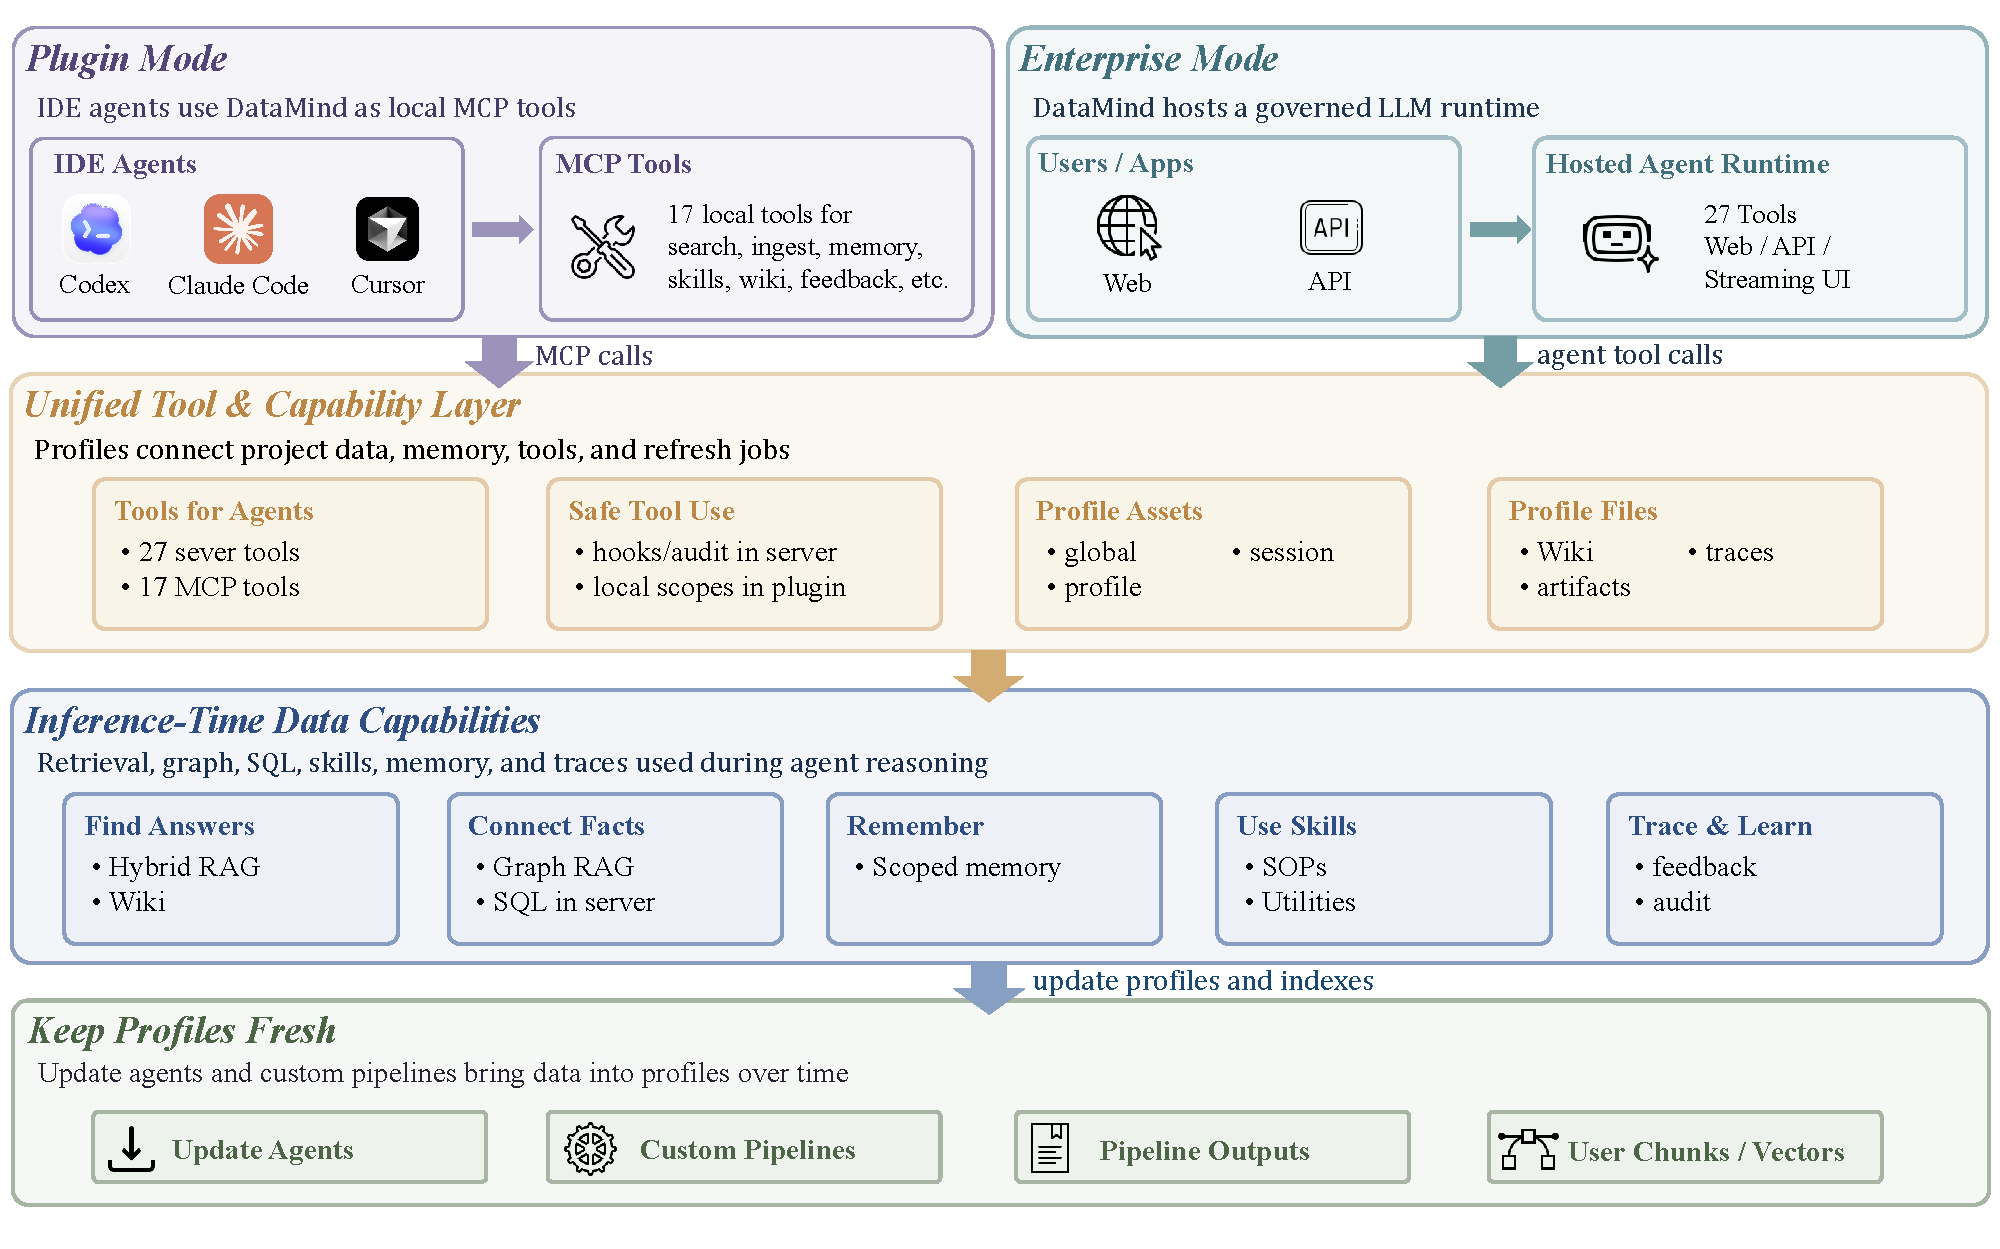
\includegraphics[width=0.94\textwidth]{figures/datamind_overview_v2.pdf}
\caption{DataMind serving path. The Serving Agent routes a request over
profile-scoped document, database, graph, memory, and skill surfaces and
returns an answer with evidence. The profile, policy, revision, and receipt
interfaces are shared with DataMind-Build.}
\label{fig:datamind-overview}
\Description{DataMind architecture showing DataMind-Build materializing workspace artifacts into document, database, and graph surfaces, while the Serving Agent routes requests over a published profile snapshot that also includes runtime memory.}
\end{figure*}

\subsection{Workspace-to-surface materialization}
\label{sec:build-agent}

DataMind-Build makes a workspace usable. Its Build Agent begins with
an inspection of profile-allowed roots and an artifact inventory. It then
selects a parser and produces provider-neutral blocks with source locators.
PDF and office documents may use a hosted document parser; a local PDF parser
is retained as a deterministic fallback. Tables are normalized into rows and
columns, while source and dependency files can contribute graph entities and
edges. The parser choice is recorded because changing a parser can change a
surface revision even when the source checksum is unchanged.

\begin{figure*}[t]
\centering
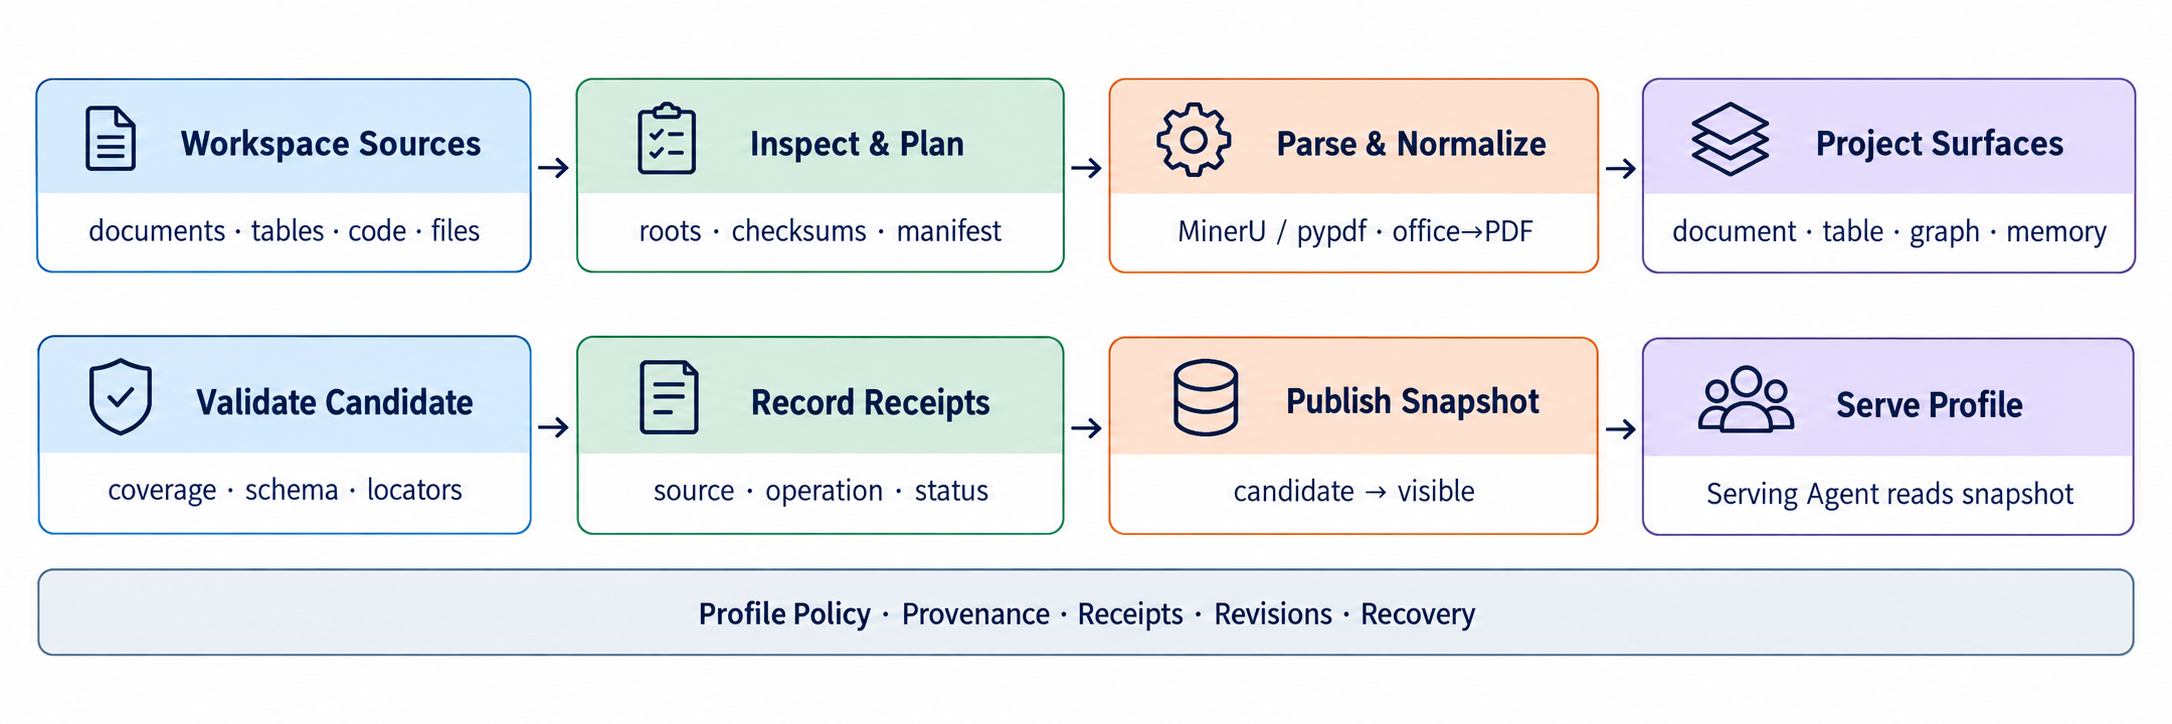
\includegraphics[width=0.94\textwidth]{figures/datamind_build_agent_generated.png}
\caption{DataMind-Build ingestion path. The Build Agent inventories a profile's
workspace, plans surface candidates, parses and normalizes sources, projects
records, validates candidate revisions, and publishes a profile snapshot. The
candidate descriptor remains unpublished until validation; reads of touched
surfaces are blocked during candidate assembly, and providers that do not
support historical artifacts fail closed if a pinned request becomes stale.}
\label{fig:datamind-build}
\Description{DataMind-Build pipeline from workspace sources through inspection,
parsing, surface projection, validation and receipts, to publication of a
profile snapshot consumed by the Serving Agent.}
\end{figure*}

The next stage projects the extracted blocks into one or more physical
surfaces. Document blocks are chunked and indexed for hybrid retrieval. Tables
are written to a relational backend with a schema that can be inspected before
query execution. Graph records are written with source annotations so a path
can be traced to the files that induced its edges. The current build path
materializes document, database, and graph surfaces; memory and skills remain
profile-scoped runtime surfaces populated by their own write tools. The Build
Agent is allowed to produce only the surfaces selected by the profile
configuration; it does not assume that every workspace needs every
representation.

Each projection emits a receipt and is validated before publication. Validation
checks include source coverage, schema shape, duplicate handling, and
surface-specific invariants such as parseable SQL tables or resolvable graph
locators. A successful build produces a manifest and a candidate snapshot. The
candidate record is outside the normal publication path until validation and
the single pointer update. During assembly, the read guard blocks the touched
surfaces so live-only providers cannot leak a partial candidate. The current
prototype does not claim that every provider stages physical files
transactionally; it reports an explicit failure when a live-only provider can
no longer satisfy a pinned record.

\subsection{Surface-to-agent serving}
\label{sec:serving-agent}

The Serving Agent receives a request together with its profile and snapshot. It
first inspects the available surface manifests. A request about a policy clause
can be answered from the document surface; a request requiring aggregation
should use a database operation; a dependency question needs the graph. A
cross-surface request produces a plan that includes the minimum set of
operations whose evidence types can jointly support the answer.

The planner does not treat all tools as equivalent. It uses operation schemas
to decide which arguments are legal and source and revision metadata to avoid
mixing incompatible views. Manifests also expose cost and freshness for
analysis and future planning; the current prototype does not implement a
cost-based optimizer.
The model remains responsible for interpreting the request and synthesizing
natural language, but the data plane controls the values and evidence that can
enter that synthesis. Intermediate results can be referenced by receipt rather
than copied verbatim through the model context. This distinction is important
for tables and graph neighborhoods that are large relative to a prompt.

When an operation fails, the Serving Agent preserves the distinction between
an empty result and an unavailable capability. An empty retrieval result is
evidence that the surface returned no matching item; an unavailable graph
store is an execution failure. The model may issue another tool call, but the
runtime does not claim an automatic cross-surface recovery planner. The trace
records the failed operation and the receipts used by any final answer.

\subsection{Updates and version visibility}
\label{sec:updates}

A source update is represented as a new source fingerprint and a new profile
revision. The ingestion ledger makes a repeated write idempotent: the same
normalized tool call and source checksum returns an unchanged receipt rather
than adding a second copy. A changed source produces a new receipt and updates
the surface-specific materialization. This ledger is deliberately separate
from the physical index so that a profile can be audited even when a backend
is replaced.

For a multi-surface build, the system records a candidate and publishes a
snapshot after validation. Serving requests pin the publication record at
request start. A provider that can open that record may continue on it; the
built-in live-only providers instead fail closed when publication advances.
While a candidate is being assembled, reads of surfaces touched by that
candidate are blocked until validation and publication complete.
This is the visibility rule used in the update experiments: stale reads are
counted as explicit failures, never as apparently successful mixed views.
Physical staging and historical reads are provider-level extensions beyond
the current prototype and are not assumed by the core claim.

\subsection{Access control and profile isolation}
\label{sec:policy}

DataMind separates update visibility from access control. Updates determine
which revision a request observes; access control determines which sources and
operations that request may access. Policy is enforced at dispatch, where a
proposed model action becomes an operation on data. Path policies resolve
symlinks and restrict file and CSV access to profile roots and configured extra
roots. SQL policies distinguish
read-only queries from destructive statements and can deny, request
confirmation, or rewrite a call. Audit records include allowed, denied, and
confirmation-required operations. The profile identifier is carried through
these checks, the capability handler, the receipt, and the final trace.

This boundary complements rather than replaces database authorization. A
backend still enforces its own permissions; DataMind prevents an Agent from
reaching an operation that the profile policy has not exposed. The same
mechanism also applies to a local MCP client and to the hosted runtime, which
keeps safety behavior independent of the model SDK.

\section{Prototype}
\label{sec:prototype}

DataMind is implemented as a protocol-oriented Python runtime. A registry maps
a surface operation to a handler, input schema, access mode, and metadata. The
agent loop sees the registry rather than a backend-specific object. The current
prototype contains a hybrid document retriever, a SQLite relational backend,
a NetworkX-backed graph store, and a SQLite-backed memory provider. Each
provider can be replaced while preserving the profile and receipt interfaces.

The implementation has two logical agents. The StoreAgent owns writes and
returns structured ingestion receipts. It routes file, folder, text, CSV,
triple, skill, and memory operations through the ingestion ledger. The
RetrieveAgent is read-only during normal chat and returns an answer, evidence,
surfaces used, and a tool trace. This division makes the read/write boundary
explicit and gives the evaluation a direct way to compare a mutable pipeline
with a snapshot-based one.

Document format adapters cover plain text, Markdown, HTML, JSON, XML, source
code, and PDF. Legacy Office documents (DOC and PPT) are converted to PDF via
LibreOffice; DOCX and PPTX use native extractors in the current prototype.
Tabular files (CSV/TSV and XLS/XLSX) are loaded into typed relations. The original file remains the
lineage source. MinerU is accessed through its hosted API when configured, and
pypdf provides a local PDF fallback. These choices affect build quality and
cost, but are not themselves the data-plane contribution.

The runtime can be used through a native model loop, a provider SDK loop, or an
MCP adapter. The adapter used by an IDE exposes the same profile directory and
surface operations as the hosted service. This makes the local plugin a
deployment surface for the data plane rather than a separate system. The
implementation section intentionally does not claim that every backend or
external pipeline is production-hardened; those claims are tested only when
the corresponding end-to-end path is included in the experiments.

\section{Evaluation}
\label{sec:experiments}

The evaluation is organized around the lifecycle in Figure~\ref{fig:datamind-overview}:
materialize workspace data, serve requests over a published view, maintain the
view under changes, and recover when a component fails. We use four research
questions:
\begin{itemize}
  \item \textbf{RQ1}: Does surface-aware serving improve route, evidence,
  answer quality, and efficiency?
  \item \textbf{RQ2}: What is the cost of building multiple surfaces, and when
  is that cost amortized by later queries?
  \item \textbf{RQ3}: Do profile snapshots and ingestion receipts preserve
  visibility, idempotence, and isolation under updates and concurrency?
  \item \textbf{RQ4}: Can DataMind recover from surface and build failures
  without returning untraceable answers?
\end{itemize}

\subsection{Workloads and baselines}
\label{sec:eval-workloads}

The main serving workload is WorkSurface-Bench. It contains auditable tasks
whose required evidence is grounded in document spans, executable table
queries, and annotated graph sources~\cite{worksurfacebench2026}. We adapt the
canonical document, table, and graph representations to DataMind surface
contracts and verify the adapter before any model run. The normal serving
agent receives no gold surface label. Gold-constrained settings are reported
only as upper bounds.

We compare DataMind with the benchmark's no-tool, document-only,
single-surface, and all-tools ReAct settings. We also implement a simple
manifest router that receives the same surface descriptions but does not use
DataMind's snapshot, evidence, or receipt path. All comparisons use the same
model backbone, prompt budget, tool schemas, task order, and temperature. The
backbone sweep follows WorkSurface-Bench (GPT-4o-mini, DeepSeek-V4-Pro,
Gemini-3.1-Pro, and GPT-5.5); the DataMind build and dynamic-system studies
fix GPT-5.5 to isolate data-plane effects. We report repeated-run means and
confidence intervals rather than a single trajectory.

\subsection{RQ1: Serving quality and efficiency}
\label{sec:eval-rq1}

The primary metrics are Route F1, Evidence, Answer, and Efficiency. We also
measure the number of accessed surfaces, operation calls, invalid calls,
irrelevant surface calls, input/output tokens, and end-to-end latency. The
analysis separates single-surface and cross-surface tasks. This distinction
prevents a system from appearing efficient merely because it avoids the hard
cases that require evidence from more than one surface.

RQ1 reports serving quality, routing behavior, evidence coverage, and runtime
cost under a fixed single-version workspace. Snapshot publication and parser
fallback are evaluated in the dynamic update and fault-injection experiments,
respectively, because a static benchmark with one valid revision and no
injected failures cannot identify their effects. If the full system improves
answer quality but increases unnecessary exploration, the additional tool and
token measurements make that trade-off explicit.

\subsection{RQ2: Build cost and amortization}
\label{sec:eval-rq2}

WorkSurface-Build begins with raw workspace artifacts and produces the surfaces
used by a fixed Worker. We compare document-only, database-only, graph-only,
an unmanaged all-surface build, heuristic demand selection, and DataMind's
managed build. The unmanaged all-surface condition uses the same configured
document, database, and graph surfaces, parsers, and physical backends as
DataMind but omits manifest-driven validation, receipts, snapshot publication,
and revision management. Build metrics include wall clock time, parser and
embedding calls, storage, source coverage, provenance
completeness, duplicate handling, and failed-stage recovery. After each build,
the same Worker answers the serving workload so that materialization quality is
not conflated with Agent behavior.

For $N$ subsequent queries, we report
\[
 C(N)=C_{\mathrm{build}}+N\cdot C_{\mathrm{serve}}.
\]
The break-even point is the smallest $N$ for which the extra build cost of a
multi-surface representation is recovered by its serving quality or cost
benefit. We also report a quality-cost curve instead of only a single
aggregate score. This is the experiment that connects WorkSurface-Build to the
DataMind claim: materialization is useful only when its cost produces durable
serving value.

\subsection{RQ3: Updates, snapshots, and concurrency}
\label{sec:eval-rq3}

We apply additions, modifications, deletions, repeated ingestion, and changed
dependency edges to a profile. Each update is followed by queries issued before,
during, and after publication. We measure visibility delay, stale-read rate,
duplicate-write rate, cross-surface snapshot consistency, and cross-profile
leakage. The comparison includes a mutable pipeline without a ledger, DataMind
without snapshot publication, and the complete system. The ablation harness
uses the same backend and driver while enabling or bypassing the repository's
ledger, SnapshotStore publication, and read guard; the full system is the only
condition that exercises all three together.

Concurrent runs use 1, 5, 20, 50, and 100 sessions. We vary same-profile reads,
cross-profile reads, concurrent writes, and mixed read/write workloads. The
system metrics are throughput, p50/p95/p99 latency, conflicts, failed calls,
peak memory, and storage growth. Correctness metrics are reported separately;
a higher throughput with stale or cross-profile results is not counted as an
improvement.

\subsection{RQ4: Failure recovery}
\label{sec:eval-rq4}

We inject parser failures, MinerU timeouts, embedding-service failures, empty document results,
database and SQL failures (timeouts, connection failures, locked or corrupted
views), graph unavailability, interrupted builds, and corrupted derived
artifacts. For each fault, we record whether the request completes,
whether its answer is correct, whether the evidence remains auditable, and how
long the structured failure or parser fallback takes. We compare retry-only,
fixed-path structured errors, and DataMind's structured errors plus the
MinerU-to-pypdf parser fallback and candidate/read guards. DataMind does not
automatically substitute one failed surface for another.

The fault matrix distinguishes unavailable data from empty data. The parser
fallback is counted as successful only if the resulting evidence satisfies the
task requirement; a plausible answer without a valid receipt is a failure.
Surface outages and stale-provider blocks are counted as explicit failures,
not as successful fallbacks. This prevents the recovery experiment from
rewarding a model for guessing after a source outage.

\subsection{Ablation and overhead}
\label{sec:eval-overhead}

A final experiment isolates runtime overhead on a local single-surface workload.
We measure manifest lookup, receipt creation, policy checks, snapshot selection,
and audit logging separately from model latency. Cold-start and warm-cache
runs are randomized, repeated, and reported with p50/p95/p99 latency and
throughput. This experiment is not intended to show that DataMind is faster
than a fixed RAG pipeline; it quantifies the cost of the semantics required for
profiles, evidence, and recovery.

\section{Related Work}
\label{sec:related}

\subsection{RAG, graph retrieval, and memory}
\label{sec:related-retrieval}

RAG grounds generation in an external corpus~\cite{lewis2020rag}, while
GraphRAG adds graph structure for query-focused retrieval and summarization
~\cite{edge2024graphrag}. Modular retrieval toolkits such as FlashRAG make it
easier to compare retrievers and indexing choices~\cite{jin2025flashrag}. These
works improve how one representation is searched. DataMind addresses the
boundary between several representations: it records how a source contributes
to a document, relational, graph, or memory surface and exposes the resulting
revision and evidence metadata to the Agent.

Long-term-memory systems such as MemGPT treat durable state as a first-class
part of an Agent architecture~\cite{packer2023memgpt}. DataMind's memory
surface is narrower: it provides profile and session scopes and integrates
memory writes with the same receipt and policy path as other surfaces. It does
not propose a new memory retrieval algorithm.

\subsection{LLM systems for data and data lakes}
\label{sec:related-data-agents}

DB-GPT demonstrates an end-to-end system for natural-language interaction with
data~\cite{xue2024dbgpt}, while SiriusBI focuses on industrial business
intelligence, multi-round dialogue, and domain-adaptive SQL generation
~\cite{jiang2025siriusbi}. Pneuma studies LLM-based representation and
retrieval for tabular data discovery~\cite{balaka2025pneuma}. NeurDB explores
an AI-powered autonomous database architecture~\cite{zhao2025neurdb}. These
systems target particular data-management experiences or database workloads.
DataMind is complementary: its unit of management is a profile containing
multiple data surfaces, and its evaluation includes the construction and
maintenance of those surfaces rather than only a database interaction task.

AOP is closer in spirit because it composes semantic operators over structured,
semi-structured, and unstructured data and studies pipeline orchestration and
optimization~\cite{wang2025aop}. DataMind differs in the lifecycle boundary it
makes explicit. AOP primarily optimizes an online semantic pipeline; DataMind
tracks the materialized surfaces, profile snapshot, source revision, and
receipts that connect an offline build to later serving and updates.

Enterprise data integration work has also shown that public benchmarks can
overestimate LLM performance on private organizational data and has proposed
annotations and ontology synthesis to close that gap~\cite{kayali2025mindgap}.
WorkSurface-Bench follows this enterprise-workload motivation, while DataMind
uses the workload to evaluate a data-plane runtime rather than a data-integration
model.

\subsection{Agent--database interfaces and workflow reliability}
\label{sec:related-reliability}

BridgeScope decomposes database access into fine-grained tools, aligns tools
with database privileges, and provides a proxy for transferring intermediate
results without routing them through the LLM~\cite{weng2026bridgescope}. These
are important database-side mechanisms. DataMind generalizes the boundary to
several surfaces and adds profile snapshots, build-time materialization, and
source-linked evidence across those surfaces.

SagaLLM applies context management, validation, and compensating transactions
to multi-agent planning workflows~\cite{chang2025sagallm}. DataMind shares the
concern for durable state and recovery but has a different state boundary: it
manages the data products that an Agent reads and writes, rather than the
business actions of a multi-agent plan. We therefore make a narrower claim
than full ACID execution for arbitrary Agent actions.

Classical provenance and workflow systems provide the conceptual basis for
source lineage, derivation, and replay~\cite{cheney2009provenance,green2007provenance}.
DataMind's challenge is to carry those ideas across vector retrieval, SQL,
graph traversal, and memory operations while exposing enough metadata for a
language model to select an operation.

\section{Conclusion}
\label{sec:conclusion}

DataMind treats a workspace used by a tool-using Agent as a managed collection
of data surfaces. The Build Agent organizes raw artifacts into document,
relational, graph, and memory representations. The Serving Agent selects and
combines those representations for a request. Profiles, snapshots, surface
contracts, receipts, policy checks, and recovery connect the two directions.

This build--serve--update--recovery view gives a concrete data-management
interpretation to multi-surface Agent workloads. WorkSurface-Bench measures
whether the serving path obtains the right surfaces and evidence; WorkSurface-
Build measures the cost and value of constructing them; dynamic experiments
measure whether the resulting view remains correct as the workspace changes.
The central claim of the paper is therefore about the data plane beneath the
Agent, not about a particular model, parser, SDK, or tool list.
